\documentclass{article}

% if you need to pass options to natbib, use, e.g.:
%     \PassOptionsToPackage{numbers, compress}{natbib}
% before loading neurips_2023

% ready for submission
\usepackage[final, nonatbib]{neurips_2023}

% to avoid loading the natbib package, add option nonatbib:
%    \usepackage[nonatbib]{neurips_2023}

\usepackage[utf8]{inputenc} % allow utf-8 input
\usepackage[T1]{fontenc}    % use 8-bit T1 fonts
\usepackage{hyperref}       % hyperlinks
\usepackage{url}            % simple URL typesetting
\usepackage{booktabs}       % professional-quality tables
\usepackage{amsfonts}       % blackboard math symbols
\usepackage{nicefrac}       % compact symbols for 1/2, etc.
\usepackage{microtype}      % microtypography
\usepackage{xcolor}         % colors

\usepackage{caption} 
\captionsetup[table]{skip=10pt}

\usepackage[spanish, es-tabla]{babel}

\usepackage[pdftex]{graphicx}
\usepackage{subcaption}
\graphicspath{{./graphs/}}

%% biblatex
\usepackage[style = numeric, backend = biber, sorting = none, doi = false, isbn = false, url = true]{biblatex}
% \usepackage[defernumbers = true, style = numeric, backend = biber, sorting = none, doi = false, isbn = false, url = true]{biblatex}
% \usepackage[style = numeric, backend = biber, sorting = none]{biblatex}    % REFERENCIAS como section
\AtEveryBibitem{
    \clearfield{urlyear}
    \clearfield{urlmonth}
} % Do not show the "(visited on <date>)" on the references
\DefineBibliographyStrings{spanish}{}
\usepackage{csquotes}
\addbibresource{./dmcyt.bib}
\renewcommand*{\bibfont}{\fontsize{9}{12}\selectfont}

\title{Clustering y segmentación de imágenes de cinco variedades de arroz mediante algoritmos no supervisados}

\author{
  Víctor A.~Bettachini\\
  \texttt{bettachini@gmail.com}
  \And Vanesa Flores\\
  \texttt{vanesaflores0894@gmail.com}
  \And Tomás Gianni\\
  \texttt{tomasgianni11@gmail.com}
  \And Malena Pirola\\
  \texttt{malenapirola@gmail.com}
}

\begin{document}


\maketitle


\begin{abstract}
La clasificación en variedades y evaluación de calidad de los granos de arroz de forma tradicional insume gran cantidad de tiempo y recursos, los cuales podrían ser optimizados mediante el uso de técnicas de análisis de imagen y aprendizaje automático. En este trabajo se evaluaron soluciones de agrupamiento no supervisado de imágenes color de granos de arroz de cinco variedades distintas mediante los algoritmos K-means, DBSCAN y Partición Alrededor de Medoides (PAM).
Las variables sobre la que se realizó el agrupamiento fueron atributos generados en una capa intermedia de la red convolucional entrenada para la clasificación de imágenes (VGG16). El desempeño de los algoritmos de agrupamiento se midió mediante métricas de validación interna y externa. En estos términos, K-means y PAM presentaron un desempeño muy similar y muy superior al de DBSCAN.
Asimismo, para ensayar la identificación de granos individuales en imágenes con muchos de estos, se realizó una segmentación con algoritmos de etiquetado de componentes conectados y de agrupamiento espectral. Para el caso de imágenes de granos de arroz bien separados, ambos algoritmos dieron resultados satisfactorios, aunque el agrupamiento espectral arrojó mejores resultados para segmentar imágenes con múltiples granos de arroz superpuestos.
\end{abstract}


    
\section{Introducción}
El arroz, uno de los granos de mayor producción en todo el mundo, tiene muchas variedades genéticas que se diferencian entre sí por atributos como la textura, la forma y el color.
Estos atributos permiten clasificar y evaluar la calidad de las semillas, lo cual afecta el precio final del producto.
Tradicionalmente, esta tarea requiere de la participación de operadores humanos expertos, con un elevado costos y tiempo de procesamiento.
La implementación de algoritmos de aprendizaje automático sobre imágenes de las semillas de arroz puede permitir una agilización del proceso de clasificación y evaluación de la calidad y un uso más eficiente de los recursos.

Se han publicado interesantes resultados en la tareas de clasificación mediante algoritmos supervisados de este tipo de imágenes.
Algunos algoritmos clásicos, e.g. Random Forest o KNN, operando con atributos morfológicos y de color alcanzaron tasas de éxito de clasificación superiores al 98\% \cite{murat_kuklu_rice_2022}, en tanto que con redes convolucionales profundas se logró una tasa de éxito del 100\% entrenando la red directamente con las imágenes \cite{koklu_classification_2021}.

Utilizando las mismas imágenes que las empleadas en éste último estudio \cite{koklu_classification_2021}, en este trabajo se busca evaluar la capacidad de agrupamiento de imágenes de semillas mediante algoritmos no supervisados a partir de atributos extraídos de una red convolucional pre-entrenada para la clasificación de imágenes \cite{simonyan_very_2015}.
Asimismo, se busca explorar las posibilidades que ofrecen diferentes algoritmos de segmentación para la identificación de granos de arroz individuales en imágenes con muchos de estos.

Es razonable suponer que si provee capacidad de caracterización de los granos a partir de sus imágenes será por su forma y color siendo insensible a la textura.
A pesar de esta limitación, que no hemos cuantificado, se emprendió la tarea de agrupar atributos obtenidos mediante la aplicación de la red convolucional utilizando distintos algoritmos de agrupación: K-Means, DBSCAN y PAM (partición alrededor de medoides). 


\section{Materiales y métodos}

\paragraph{Datos}
Se obtuvieron de una fuente pública \cite{murat_kuklu_rice_2022} unas 75K imágenes de granos de arroz balanceadas en 5 distintas variedades (15K imágenes por cada tipo): Arborio, Basmati, Ipsala, Jazmín y Karacadag, que corresponden a variedades que suelen cultivarse en Turquía.
Las imágenes provistas en formato jpeg presentan tres capas de color RGB (rojo, verde y azul) con un tamaño de 250 x 250 píxeles.
Cada píxel tiene un valor de 0 a 255 que codifica la intensidad lumínica del color.
En cada imagen se visualiza un único grano de arroz que está centrado en la imagen sobre un fondo negro, como se observa en los ejemplos (Figura \ref{fg_ejemplos}).
El procesamiento y análisis de datos se realizó sobre una muestra aleatoria estratificada sin reemplazo de 5K imágenes, i.e. 1K por cada variedad de arroz. 

\begin{figure} [!htb]
	\centering
	\begin{subfigure}[b]{0.18\textwidth}
		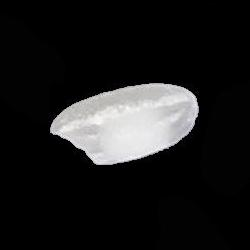
\includegraphics[width= \textwidth]{fg/Arborio.jpg}
		\caption{Arborio}
	\end{subfigure}
	\begin{subfigure}[b]{0.18\textwidth}
		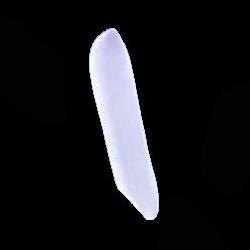
\includegraphics[width= \textwidth]{fg/Basmati.jpg}
		\caption{Basmati}
	\end{subfigure}
	\begin{subfigure}[b]{0.18\textwidth}
		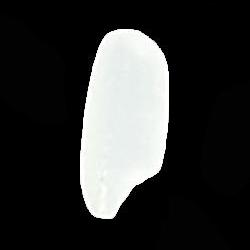
\includegraphics[width= \textwidth]{fg/Ipsala.jpg}
		\caption{Ipsala}
	\end{subfigure}
	\begin{subfigure}[b]{0.18\textwidth}
		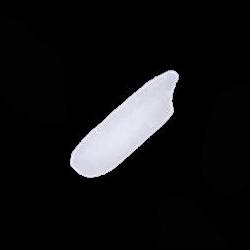
\includegraphics[width= \textwidth]{fg/Jasmine.jpg}
		\caption{Jazmín}
	\end{subfigure}
	\begin{subfigure}[b]{0.18\textwidth}
		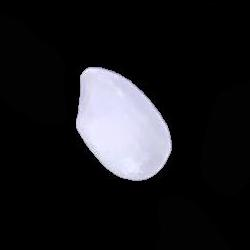
\includegraphics[width= \textwidth]{fg/Karacadag.jpg}
		\caption{Karacadag}
	\end{subfigure}
	\caption{Ejemplo de imagen del conjunto de datos para cada variedad de arroz representada [a) - e)].}	
\label{fg_ejemplos}
\end{figure}


\paragraph{Extracción de atributos} 
% \paragraph{Pre-procesamiento y extracción de atributos} 
Para lograr una reducción de la dimensionalidad de los datos de cada imagen se empleó un modelo provisto por la biblioteca Keras bajo el nombre VGG16 \cite{team_keras_nodate}.
Este es producto de entrenar una red convolucional de 16 capas en forma supervisada para la clasificación de imágenes \cite{simonyan_very_2015}.
Neuronas de sus capas intermedias responden a atributos abstractos útiles para realizar tareas distintas a la clasificación y/o trabajar sobre imágenes disímiles a las usadas en el entrenamiento (\textit{transfer learning}).
Así se caracterizan distintos aspectos abstraídos de la imagen que pueden ser utilizados para entrenar algoritmos de clasificación o agrupamiento más específicos a cierto dominio (\textit{fine-tuning}).  

Cada imagen se redujo a 224 x 224 píxeles que se ordenaron en un vector único de tamaño 150.528 (224 x 224 x 3).
Tras alimentar cada una de ellas se registró la salida de la penúltima capa que consta de 4.096 neuronas, obteniéndose una reducción al \(\approx 2.7\%\) de su dimensionalidad original.
 

\paragraph{Clustering} 
Los 4.096 atributos de cada imagen, previamente normalizados entre 0 y 1 a través del método MinMax, se alimentaron a tres distintos algoritmos no supervisados de agrupación (\textit{clustering}): K-means, DBSCAN y PAM (o K-medoides).  
Se evaluaron los resultados con medidas de validez interna y externa.

El algoritmo de K-means opera en una serie de pasos. 
\begin{enumerate}
  \item Selecciona un número predefinido de clusters (K) y elige K puntos iniciales como centros de los clusters de manera aleatoria.
  \item Asigna cada punto de datos al cluster cuyo centro está más cercano, generalmente utilizando la distancia euclidiana.
  \item Calcula el nuevo centro de cada cluster como el promedio de los puntos asignados a ese cluster.
  \item Repite los pasos 2 y 3 hasta que los centros de los clusters converjan o hasta que se alcance un número máximo de iteraciones predefinido.
\end{enumerate}
El resultado final del algoritmo es un conjunto de K clusters, donde los puntos de datos dentro de cada cluster son similares entre sí y diferentes de los puntos en otros clusters.

El algoritmo DBSCAN (\textit{Density-Based Spatial Clustering of Applications with Noise}) es un método de agrupamiento que, a diferencia de K-means, no requiere que se especifique previamente el número de clusters (k).
En su lugar, DBSCAN identifica clusters basándose en la densidad de puntos en el espacio de datos.
Detecta automáticamente la cantidad de clusters y es especialmente efectivo para encontrar clusters de formas arbitrarias y separados por áreas de baja densidad.
DBSCAN también puede manejar ruido de manera más efectiva al clasificar puntos ruidosos como ruido en lugar de asignarlos a un cluster, lo que lo diferencia de K-means en términos de robustez en datos reales y la capacidad de adaptarse a la estructura de los datos sin requerir suposiciones iniciales sobre el número de clusters.

El algoritmo PAM (\textit{Partitioning Around Medoids}), también conocido como K-medoids, es similar a K-means, pero se diferencia de éste en su enfoque en la elección de los puntos representativos del cluster.
En lugar de usar la media de los puntos como centro del cluster (como en K-means), PAM selecciona medoides, que son puntos reales del conjunto de datos.
Estos medoides son los puntos que minimizan la distancia total a todos los demás puntos dentro del cluster.
Esta estrategia hace que PAM sea más robusto frente a valores atípicos o ruidosos en comparación con K-means y permite una interpretación más clara de los puntos representativos de cada cluster.

Las medidas de validez interna empleadas para evaluar los algoritmos fueron el SSE y el coeficiente de Silhouette.
El primero es la suma de los cuadrados de las distancias de cada observación al centroide del cluster (más bajo cuanto más compactos y coherentes sean los clusters). 
El segundo cuantifica entre -1 y 1 cuán similar es cada punto de datos a su propio cluster comparándolo con otros clusters cercanos.
Cuánto menor sea el coeficiente de Silhouette, más grande es la diferencia entre el punto y otros miembros del cluster, indicando que el punto está "mal agrupado", mientras que valores en torno a 0 sugieren un gran solapamiento entre los grupos.
Estas dos medidas de validez interna también son útiles para determinar la cantidad óptima de clusters.
Para esto se aplicaron iterativamente para los casos de 1 a n clusters y luego se compararon los resultados medidos por SSE y Silhouette. 

Por otro lado, la validación externa permite comparar diferentes soluciones de agrupamiento entre sí. Se calculó una la matriz de confusión agrupando variedades de arroz según la etiqueta en el conjunto de datos vs. al cluster asignado por los algoritmos.
Esto permitió evaluar cuán bien mapearon los clusters las variedades y la utilidad de dichos algoritmos para su separación. Asimismo, se calculó el índice de Rand ajustado, que puede tomar valores entre 0 y 1 donde 1 indica una concordancia perfecta entre las asignaciones de clústeres y 0 indica una asignación aleatoria. Además, se calculó el índice de van Dongen, que cuantifica la disimilaridad entre clusters basada también en la intersección máxima de clusters y toma valor 0 cuando los clusters son iguales entre ambas soluciones de agrupamiento.


\paragraph{Segmentación}
Para realizar la segmentación y detección de objetos individuales se sintetizó una imagen nueva a partir de cuatro imágenes de granos de arroz de diferente variedad. 
La imagen resultante fue de 500 x 500 pixeles con 3 canales de color, la cual fue pasada a blanco y negro utilizando la función umbral de la biblioteca OpenCV para Python con un valor de 0 (i.e. todos los pixeles con valor superior a 0 fueron llevados a 255).
Como evaluación adicional, se aplicaron los algoritmos de segmentación sobre una imagen adicional obtenida de la web con muchos granos de arroz.

Se aplicaron dos algoritmos de segmentación: a) etiquetado de componentes conectados (CCL, por sus siglas en inglés) utilizando la librería OpenCV, y b) clustering espectral mediante la librería Scikit-learn (\verb'sklearn.clustering') para Python.
CCL es un algoritmo iterativo que parte de examinar un pixel, que oficia de ``semilla'' y luego examina sus pixeles vecinos.
Si éstos tienen características similares al pixel semilla, se lo considera parte del mismo componente, de lo contrario se lo considera un componente diferente.
De esta manera se recorren todos los píxeles de la imagen hasta que todos se asignan a algún componente.
Por otro lado, el clustering por análisis espectral parte de la generación de una matriz de similaridad entre los puntos que sirve de base para crear un grafo, en donde cada punto es un nodo y las similitudes son las aristas que los conectan, con menor o mayor ``fuerza'' según el grado de similitud entre los puntos.
Mediante la descomposición en autovectores y autovalores de las matrices asociadas con el grafo, el algoritmo es capaz de agrupar puntos que están fuertemente conectados y separarlos de otros grupos.  


\section{Resultados}

\paragraph{Clustering por K-means}
Se analizaron los gráficos de las medidas de validez interna para los clusters en función del número de los mismos.

Para el caso del SSE puede notarse en la figura \ref{fg_kmeans_valint_sse} que disminuye en forma suave, sin presentar un quiebre que indique de forma obvia la cantidad de clusters óptimo.
Esto puede deberse a que los atributos no poseen una clara estructura de agrupamiento.

En el caso del coeficiente de Silhouette la figura \ref{fg_kmeans_valint_silhoutte} muestra que este resultó cercano a 0 para todos los números de clusters seleccionados (k).
Por tanto calculare este coeficiente no proveyó una guía clara de que que número sería el adecuado.

\begin{figure} [!htb]
	\centering
	\begin{subfigure}[b]{0.45\textwidth}
		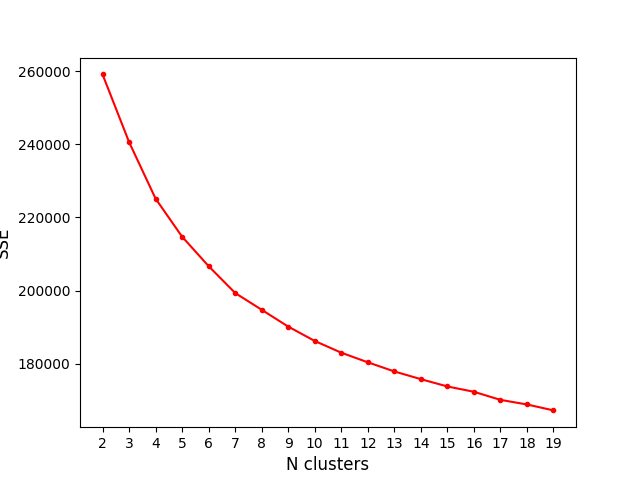
\includegraphics[width= \textwidth]{fg/kmeans_sse (1).png}
        \caption{SSE}
		\label{fg_kmeans_valint_sse}
	\end{subfigure}
	\begin{subfigure}[b]{0.45\textwidth}
		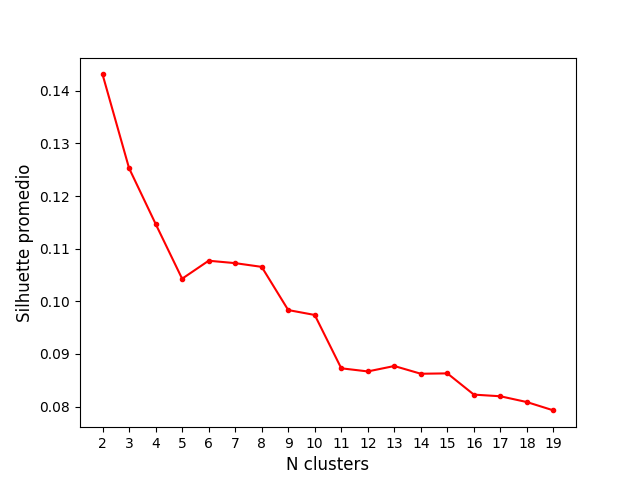
\includegraphics[width= \textwidth]{fg/kmeans_silhouette (2).png}
        \caption{Coeficiente de Silhouette promedio vs. clusters}
        \label{fg_kmeans_valint_silhoutte}
	\end{subfigure}
	\caption{K-means: métricas de validación interna.}	
\end{figure}

Considerando el objetivo del presente trabajo, se decidió proceder con \(k = 5\) clusters para evaluar la capacidad del algoritmo de agrupar las imágenes de forma comparable con las variedades de arroz originales, así como \(k = 7\) clusters para fines comparativos. 

Las medidas de validación externa que figuran en la tabla \ref{tab:kmeans} sugieren que no existen prácticamente diferencias en el desempeño en los algoritmos para cinco o siete clusters.
En la misma tabla figuran también los valores numéricos de las validaciones internas.
Para ambos números de clusters, el índice Rand ajustado sugiere que si bien los modelos no se ajustan perfectamente a la categorización por variedades conocida, la agrupación modelada es superior a la que se obtendría por azar.
Asimismo, el índice van Dongen cercano a 0 indica que para ambos modelos la solución de agrupamiento alcanzada es similar a la que resulta del agrupamiento por las etiquetas conocidas de variedad de arroz.

\begin{table}[!htb]
  \centering
  \begin{tabular}{lcccc}
    \toprule
    Clusters (k) & SSE & Silhouette promedio & Rand ajustado & van Dongen\\
    \midrule
    5 &  214744.0 &  0.1040&  0.4230& 0.1880\\ 
    7 &  199367.0&  0.1070&  0.4768& 0.1520\\
    \bottomrule
  \end{tabular}
  \caption{K-means: métricas de validez interna y externa (vs. etiquetas de clase conocidas).}
  \label{tab:kmeans}
\end{table}

La matriz de confusión del modelo de cinco clusters que presenta la tabla \ref{tab:mc_kmeans5} evidencia que al menos el tipo de arroz Karacadag quedó agrupado casi en su totalidad un sólo cluster, el numerado con 0. 
Por el contrario, los clusters 1 y 2 están compuestas por similares proporciones de Arborio e Ipsala, patrón que se repite en los clusters 3 y 4 con Jazmín y Basmati.
En la figura \ref{fg:ejemplos_clusters} se puede observar que estas agrupaciones responden a patrones de morfología de los granos que hacen difícil su separabilidad.

\begin{table}[!htb]
    \centering
    \begin{tabular}{cccccc}
    \toprule
    Cluster | Variedad &  Arborio &  Ipsala &  Jazmín &  Karacadag & Basmati\\
    \midrule
    0 & 81 & 4& 1 & 921 & 0 \\
    1 & 10 & 7& 525 & 0 & 437 \\
    2 & 456 & 468 & 40 & 22& 0 \\
    3 & 446 & 520 & 42 & 57& 1 \\
    4 & 7 & 1 & 392 & 0 & 562 \\
    \bottomrule
    \end{tabular}
    \caption{K-means: matriz de confusión para 5 clusters vs. etiquetas de variedad.}
    \label{tab:mc_kmeans5}
\end{table}

\begin{figure} [!htb]
	\centering
	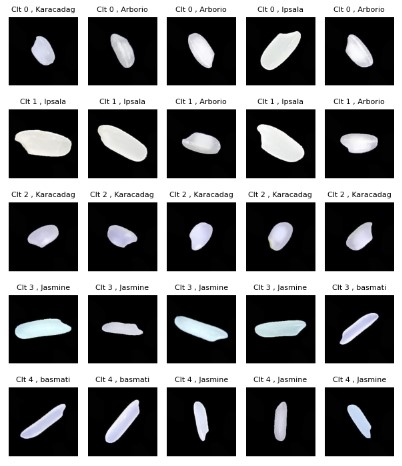
\includegraphics[width= 0.9\textwidth]{fg/ejemplos_clusters.jpg}
	\caption{K-means: ejemplos de cada uno de los cinco clusters con su etiqueta original.}	
    \label{fg:ejemplos_clusters}
\end{figure}


Como medio de facilitar la visualización de los clusters generados por K-means (k = 5), se realizó un análisis de componentes principales para reducir la dimensionalidad del espacio de atributos.
La figura \ref{fg:pca} muestra los cinco clusters graficados sobre los componentes 1 y 2 obtenidos mediante PCA (+40\% de variabilidad explicada), en donde se corrobora cierta superposición entre los grupos y por ende, baja separabilidad.

\begin{figure} [!htb]
	\centering
	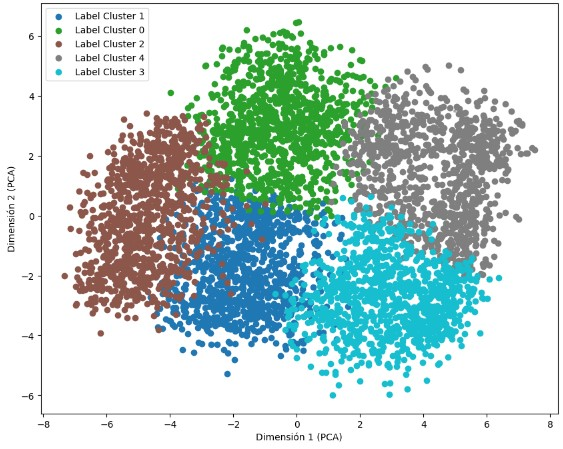
\includegraphics[height= 8.0 cm]{fg/PCA_clusters.jpg}
	\caption{K-means: visualización de los 5 clusters generados. Componentes 1 y 2 obtenidos por PCA sobre atributos originales utilizados para el entrenamiento).}	
    \label{fg:pca}
\end{figure}

El caso con siete clusters, que resume la tabla \ref{tab:mc_kmeans7}, volvió a verificarse la eficiente distinción de la variedad Karacadag donde el cluster 2 se compone casi exclusivamente de esta variedad, pero el resto de los clusters presenta características mixtas.

\begin{table}
    \centering
    \begin{tabular}{cccccc}
    \toprule
    Cluster | Variedad &  Arborio&  Ipsala&  Jazmín&  Karacadag& Basmati\\
    \midrule
    0 & 13 & 2 & 375 & 0 & 230 \\
    1 & 41 & 503 & 5 & 4 & 0 \\
    2 & 59 & 3 & 1 & 866 & 0 \\
    3 & 2 & 0 & 33 & 0 & 451 \\
    4 & 645 & 44 & 13& 128 & 1 \\
    5 & 11 & 8 & 537 & 0 & 318 \\
    6 & 229 & 440 & 36 & 2 & 0 \\
    \bottomrule
    \end{tabular}
    \caption{K-means: matriz de confusión para 7 clusters vs. etiquetas de variedad.}
    \label{tab:mc_kmeans7}
\end{table}


\paragraph{Clustering por DBSCAN}
Para este algoritmo se optimizaron dos parámetros, \textit{eps}, el radio del entorno usado para definir los clusters, y \textit{MinPts}, la cantidad mínima de puntos en el entorno.

En una primer instancia, se tomó un criterio sugerido en bibliografía consultada para la optimización de los parámetros: considerar el 4to vecino más cercano para realizar los agrupamientos; con dicha premisa, que equivale a establecer  \textit{MinPts} = 4 en el modelo, se corrió el algoritmo de vecinos más cercanos \textit{(KNN)} para \(n = 4\), y se buscó un quiebre en la curva representada en la figura \ref{fg_dbscan_codo}, que marca un valor de \textit{eps} óptimo de \(7,25\).

Al ajustar nuestro modelo con estos parámetros se identificó un único gran cluster y puntos ruidosos, lo cual no es satisfactorio; por ello, decidimos evaluar un rango de valores para ambos parámetros y evaluar el coeficiente de Silhouette obtenido con cada una de dichas combinaciones. Éstos resultaron muy cercanos a cero para cualquier par de parámetros \textit{eps} y \textit{MinPts} evaluados, como muestra la figura \ref{fg_dbscan_silhouette}, lo cual es indicativo de un ``mal'' agrupamiento.
Sin embargo, considerando el objetivo del presente trabajo, se decidió continuar con la combinación de parámetros que encontró cinco clusters (\textit{eps} = 6, \textit{MinPts} = 3) para evaluar la capacidad del algoritmo de agrupar las imágenes de forma comparable con las variedades de arroz originales. 

\begin{figure} [!htb]
	\centering
	\begin{subfigure}[b]{0.435\textwidth}
		\includegraphics[width= \textwidth]{fg/dbscan_codo.png}
        \caption{Distancia al 4to vecino}
		\label{fg_dbscan_codo}
	\end{subfigure}
	\begin{subfigure}[b]{0.45\textwidth}
		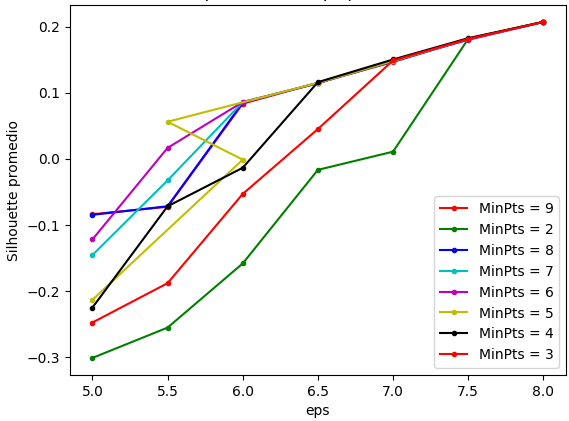
\includegraphics[width= \textwidth]{fg/dbscan_silhouette.png}
        \caption{Coeficiente de Silhouette vs. eps y MinPts}
        \label{fg_dbscan_silhouette}
	\end{subfigure}
	\caption{DBSCAN: optimización de parámetros y validación interna.}	
    \label{fg:dbscan}
\end{figure}

Las medidas de validación externa resumidas en la tabla \ref{tab:dbscan} sugieren, del mismo modo, un agrupamiento poco efectivo: tanto el índice Rand ajustado çomo el índice van Dongen indican una mala coincidencia entre lo obtenido por el modelo y las etiquetas reales de los datos.

\begin{table}[!htb]
  \centering
  \begin{tabular}{lcccc}
    \toprule
    Parámetros & Clusters & Silhouette promedio & Rand ajustado & van Dongen\\
    \midrule
    eps = 8, MinPts = 9 & 1 &  0.201 &  0 & 0.8\\ 
    eps = 86, MinPts = 3 & 5 &  -0.05 &  0.006 & 0.67 \\
    \bottomrule
    \end{tabular}
    \caption{DBSCAN: métricas de validez interna y externa (vs. etiquetas de clase conocidas).}
    \label{tab:dbscan}
\end{table}

La matriz de confusión del modelo para cinco clusters \ref{tab:mc_dbscan} refuerza estas conclusiones: se aprecia que el cluster 0 abarca la gran mayoría de los puntos, y que evidentemente los 4 clusters restantes han sido completamente forzados; el cluster -1 corresponde a los puntos que el modelo catalogó como "ruido", es decir, sin agrupamiento claro. En la figura \ref{fg:DBSCAN_ejemplos_cluster} se puede observar las agrupaciones que realizó el modelo: solo para el cluster 0 detectó al menos 10 elementos, lo cual es suficiente prueba de su baja eficiencia debido a la poca separabilidad de los datos.

\begin{table}
    \centering
    \begin{tabular}{cccccc}
    \toprule
    Cluster | Variedad &  Arborio &  Ipsala &  Jazmín &  Karacadag & Basmati \\
    \midrule
    -1 & 120 & 238 & 106 & 50 & 52 \\
    0 & 880 & 746 & 894 & 950 & 948 \\
    1 & 0 & 6 & 0 & 0 & 0 \\
    2 & 0 & 3 & 0 & 0 & 0 \\
    3 & 0 & 4 & 0 & 0 & 0 \\
    4 & 0 & 3 & 0 & 0 &0 \\
    \bottomrule
    \end{tabular}
    \caption{DBSCAN: matriz de confusión para 5 clusters vs. etiquetas de variedad.}
    \label{tab:mc_dbscan}
\end{table}

\begin{figure} [!htb]
	\centering
	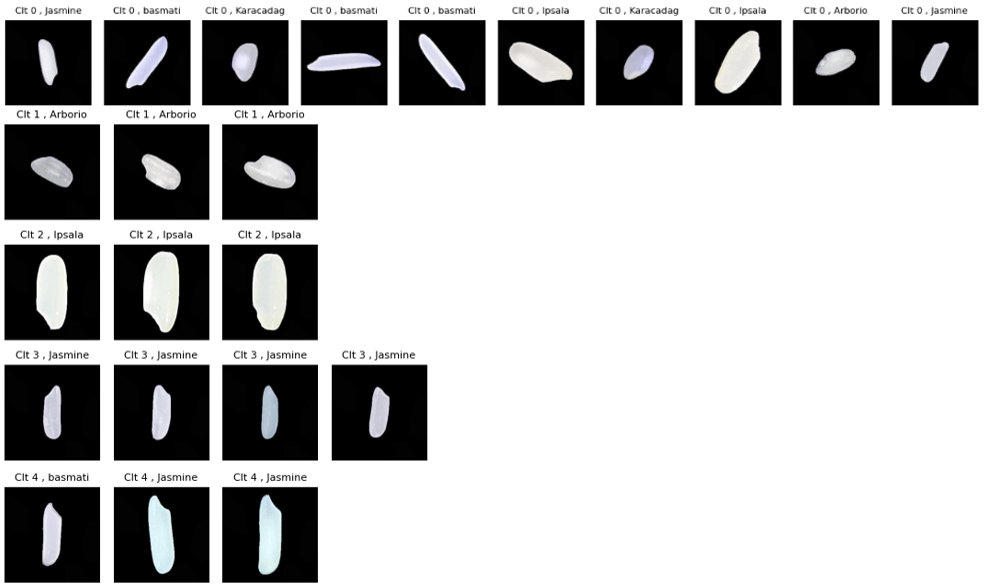
\includegraphics[height= 8.0 cm]{fg/DBSCAN_ejemplos_cluster.png}
	\caption{DBSCANs: muestra de los clusters generados}	
    \label{fg:DBSCAN_ejemplos_cluster}
\end{figure}

La figura \ref{fg:PCA_DBSCAN} muestra los cinco clusters graficados sobre los componentes 1 y 2 obtenidos mediante PCA (+40\% de variabilidad explicada), en donde se corrobora una total superposición entre los grupos y la nula separabilidad que advirtieron los resultados.

\begin{figure} [!htb]
	\centering
	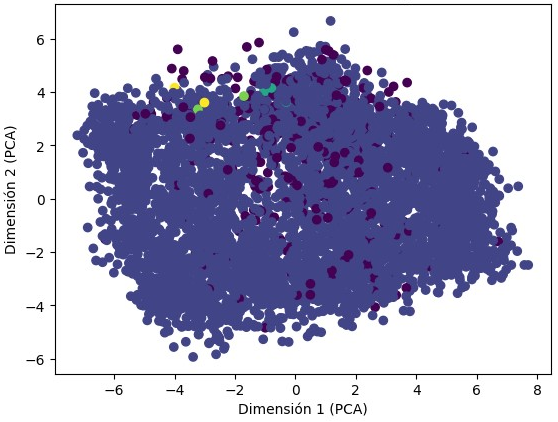
\includegraphics[height= 8.0 cm]{fg/PCA_clusters_DBSCAN.png}
	\caption{DBSCANs: visualización de los 5 clusters generados. Componentes 1 y 2 obtenidos por PCA sobre atributos originales utilizados para el entrenamiento). Hay una nula separación entre clusters.}	
    \label{fg:PCA_DBSCAN}
\end{figure}



\paragraph{Clustering por PAM}
Finalmente, probaremos el rendimiento del método de clustering \textit{PAM (Partition Aroud Medoids)}, o también conocido como \textit{K-medoids} para evaluar sus diferencias de desempeño respecto de los otros algoritmos empleados.

Al igual que lo realizado para K-means, se analizaron los gráficos de las medidas de validez interna para los clusters en función del número de los mismos: 

\begin{figure} [!htb]
	\centering
	\begin{subfigure}[b]{0.45\textwidth}
		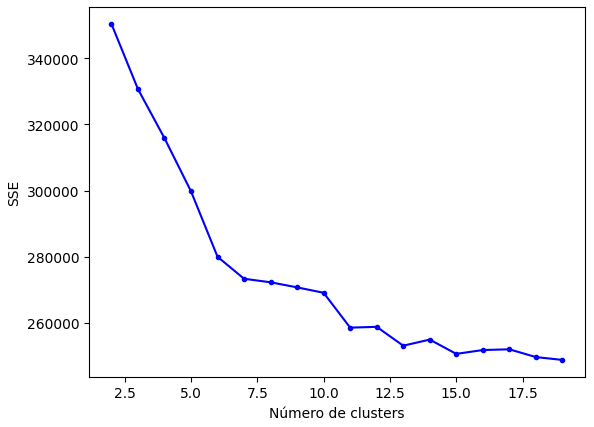
\includegraphics[width= \textwidth]{fg/PAM_sse.png}
        \caption{SSE}
		\label{fg_pam_valint_sse}
	\end{subfigure}
	\begin{subfigure}[b]{0.45\textwidth}
		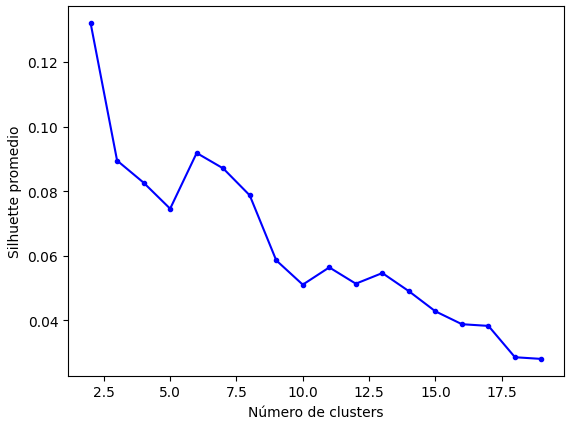
\includegraphics[width= \textwidth]{fg/PAM_silhouette.png}
        \caption{Coeficiente de Silhouette promedio vs. clusters}
        \label{fg_pam_valint_silhouette}
	\end{subfigure}
	\caption{PAM: métricas de validación interna.}	
\end{figure}

Similar a lo que ocurre con K-means, de la figura \ref{fg_pam_valint_sse} podemos notar que el valor de SSE disminuye mientras aumenta la cantidad de clusters, aunque de forma menos suave que en el primero modelo.
El quiebre de la curva alrededor de los 5 o 6 clusters permite suponer que en ese entorno se encontrará el valor óptimo.

En el caso del coeficiente promedio de Silhouette, la figura \ref{fg_pam_valint_silhouette} también muestra un comportamiento similar a K-means: el coeficiente resultó cercano a 0 para todos los números de clusters seleccionados (k).
Por tanto, calcular este coeficiente no proveyó una guía clara de qué número sería el adecuado.

A fin de realizar una comparación fructífera entre distintos algoritmos de agrupamiento, se decidió proceder con los mismos criterios que los empleados al realizar k-means: evaluar el modelo con \(k = 5\), emulando las variedades de arroz originales, así como con \(k = 7\) clusters para fines comparativos. 

Las medidas de validación externa que figuran en la tabla \ref{tab:PAM} sugieren que no existen diferencias significativas en el desempeño en los algoritmos para cinco o siete clusters, similar a lo ocurrido con K-means.
En dicha tabla figuran también los valores numéricos de las validaciones internas.
Para ambos números de clusters, el índice Rand ajustado sugiere que si bien los modelos no se ajustan perfectamente a la categorización por variedades conocida, la agrupación modelada es superior a la que se obtendría por azar. Cabe destacar que para cinco clusters éste índice fue ligeramente superior (beneficioso) que el obtenido al realizar K-means, mientras que se dio la situación inversa para 7 clusters.
Asimismo, el índice van Dongen cercano a 0 indica que para ambos modelos la solución de agrupamiento alcanzada es similar a la que resulta del agrupamiento por las etiquetas conocidas de variedad de arroz; al comparar con lo obtenido con K-means, se da una situación completamente análoga a lo descrito para el índice de Rand ajustado.

\begin{table}[!htb]
  \centering
  \begin{tabular}{lcccc}
    \toprule
    Clusters (k) & SSE & Silhouette promedio & Rand ajustado & van Dongen\\
    \midrule
    5 &  299729.0 &  0.0746&  0.4357& 0.1831\\ 
    7 &  273286.0&  0.0871&  0.4244& 0.1674\\
    \bottomrule
  \end{tabular}
  \caption{PAM: métricas de validez interna y externa (vs. etiquetas de clase conocidas).}
  \label{tab:PAM}
\end{table}

La matriz de confusión del modelo de cinco clusters que presenta la tabla \ref{tab:mc_PAM5} evidencia que el tipos de arroz Karacadag fue clasificado casi en su totalidad en el cluster 2;  el tipo Basmati también fue predominantemente agrupado en el cluster 0, pero en él también se incluyó una cantidad notable de imágenes del tipo Jasmine.
Por el contrario, los clusters 1, 3 y 4 no tienen una tan marcada superioridad de algún tipo de arroz: podemos notar, no obstante, que componen mayormente de los tipos Jasmine, Ipsala y Arborio, respectivamente. Al igual que lo ocurrido al aplicar K-means, estas agrupaciones responden a patrones morfológicos de los granos que hacen difícil su separabilidad.

\begin{table}[!htb]
    \centering
    \begin{tabular}{cccccc}
    \toprule
    Cluster | Variedad &  Arborio &  Ipsala &  Jazmín &  Karacadag & Basmati\\
    \midrule
    0 & 5 & 17 & 387 & 0 & 919 \\
    1 & 96 & 128 & 441 & 7 & 43 \\
    2 & 91 & 14 & 0 & 925 & 0 \\
    3 & 403 & 530 & 36 & 17 & 3 \\
    4 & 405 & 311 & 136 & 51 & 35 \\
    \bottomrule
    \end{tabular}
    \caption{PAM: matriz de confusión para 5 clusters vs. etiquetas de variedad.}
    \label{tab:mc_PAM5}
\end{table}

De la misma manera a lo realizado en los algoritmos anteriores, se realizó un análisis de componentes principales para reducir la dimensionalidad del espacio de atributos (k =5) y poder graficar los clusters hallados por el algoritmo PAM.
La figura \ref{fg_PCA_clusters_PAM} muestra los cinco clusters graficados sobre los componentes 1 y 2 obtenidos mediante PCA (+40\% de variabilidad explicada): se aprecia una situación intermedia entre los casos graficados para los dos algoritmos anteriores, con clusters relativamente identificables, pero también muy superpuestos, resultando en baja separabilidad.

\begin{figure} [!htb]
	\centering
	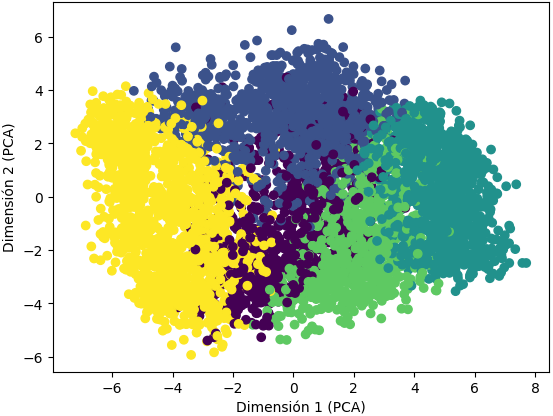
\includegraphics[height= 8.0 cm]{fg/PCA_clusters_PAM.png}
	\caption{PAM: visualización de los 5 clusters generados. Componentes 1 y 2 obtenidos por PCA sobre atributos originales utilizados para el entrenamiento.}	
    \label{fg_PCA_clusters_PAM}
\end{figure}

El caso con siete clusters, que resume la tabla (\ref{tab:mc_PAM7}), se comprueba nuevamente la eficiente distinción de las variedades Karacadag (cluster 2, compuesto casi exclusivamente de esta variedad) y Basmati (cluster 0, también casi exclusivamente); el resto de los clusters presenta características mixtas.

\begin{table}
    \centering
    \begin{tabular}{cccccc}
    \toprule
    Cluster | Variedad &  Arborio&  Ipsala&  Jazmín&  Karacadag& Basmati\\
    \midrule
    0 & 0 & 0 & 36 & 0 & 584 \\
    1 & 12 & 33 & 379 & 0 & 45 \\
    2 & 68 & 13 & 0 & 891 & 0 \\
    3 & 264 & 213 & 26 & 7 & 1 \\
    4 & 378 & 318 & 16 & 50 & 3 \\
    5 & 3 & 26 & 533 & 0 & 367 \\
    6 & 275 & 397 & 10 & 52 & 0 \\
    \bottomrule
    \end{tabular}
    \caption{PAM: matriz de confusión para 7 clusters vs. etiquetas de variedad.}
    \label{tab:mc_PAM7}
\end{table}


\paragraph{Segmentación por etiquetado de componentes conectados}

La imagen original alimentada al algoritmo contenía cuatro granos de arroz, los cuales fueron correctamente identificados como objetos separados entre sí y en relación al fondo como puede apreciarse en las figuras \ref{fg:ccl} (a - d).
El algoritmo identificó los recuadros delimitadores de cada grano (\textit{bounding box}) y su centroide en forma correcta.
Al aplicarse a la imagen adicional de múltiples granos de arroz superpuestos obtenida de la web (figura \ref{fg:ccl_web}, el algoritmo resultó en la detección de más de 90 componentes.
Esto sólo uno representa la mayor parte de los granos presentes en la foto, sin distinción entre ellos como muestra la figura \ref{fg:ccl_web_separada}.

\begin{figure} [!htb]
	\centering
	\begin{subfigure}[b]{0.2\textwidth}
		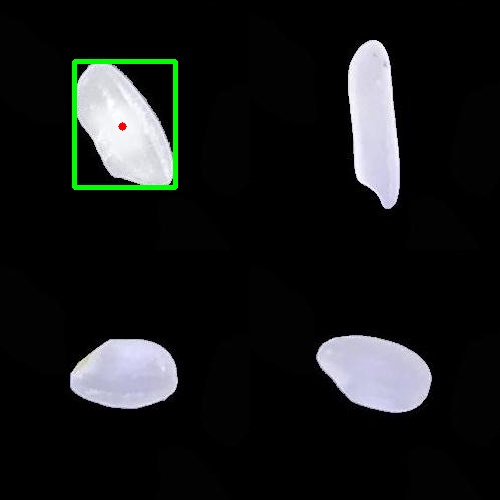
\includegraphics[width= \textwidth]{fg/ccl_bbox_centroid_2.jpg}
        \caption{}
	\end{subfigure}
	\begin{subfigure}[b]{0.2\textwidth}
		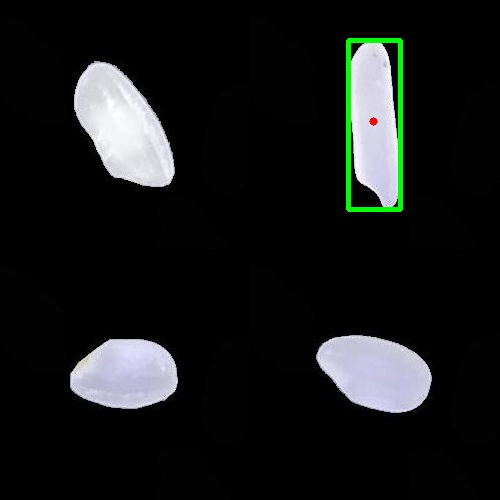
\includegraphics[width= \textwidth]{fg/ccl_bbox_centroid_1.jpg}
        \caption{}
	\end{subfigure}
	\begin{subfigure}[b]{0.2\textwidth}
		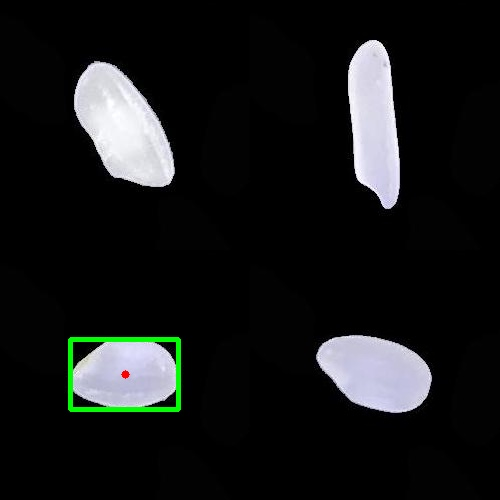
\includegraphics[width= \textwidth]{fg/ccl_bbox_centroid_4.jpg}
        \caption{}
	\end{subfigure}
    \begin{subfigure}[b]{0.2\textwidth}
		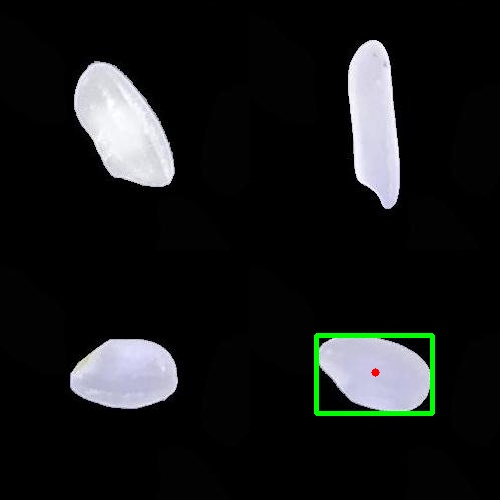
\includegraphics[width= \textwidth]{fg/ccl_bbox_centroid_3.jpg}
        \caption{}
	\end{subfigure}
      \begin{subfigure}[b]{0.2\textwidth}
		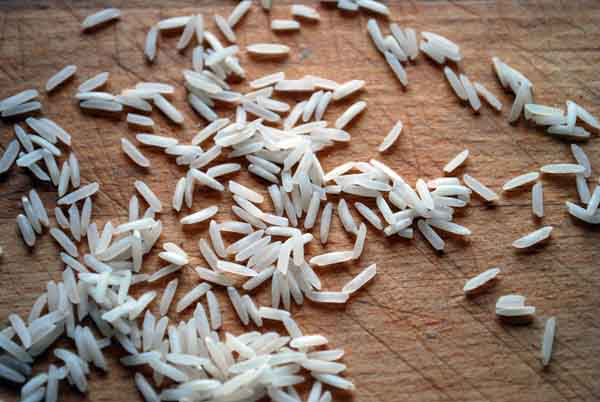
\includegraphics[width= \textwidth,height= 2.5 cm]{fg/muchos_basmati.jpg}
        \caption{}
        \label{fg:ccl_web}
	\end{subfigure}
     \begin{subfigure}[b]{0.2\textwidth}
		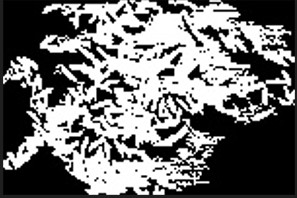
\includegraphics[width= \textwidth,height= 2.5 cm]{fg/ccl_muchos_basmati.jpg}
        \caption{}
        \label{fg:ccl_web_separada}
	\end{subfigure}
	\caption{Detección de objetos en una imagen mediante etiquetado de componentes conectados. En rojo, centroide de cada objeto y en verde, recuadro delimitador (a-d). e) Imagen de muchos granos de arroz obtenida de la web y f) recorte de 1 de los 94 componentes etiquetados para la imagen.}	
\label{fg:ccl}
\end{figure}


\paragraph{Segmentación por análisis espectral}

Para métodos de segmentación por análisis espectral se ensayaron diferentes estrategias de descomposición en autovalores.
So logró el mejor resultado con el método de gradiente conjugado precondicionado de bloque localmente óptimo local o \textit{lobpcg} \cite{knyazev_toward_2001}.
Con este se obtuvo una correcta identificación de los cuatro granos de arroz en la imagen y su diferenciación con el fondo, tal como puede apreciarse en la figura \ref{fg:espectral_granos}.
En la imagen obtenida de la web (figura \ref{fg:espectral_web}), el mejor resultado se obtuvo con ``arpack'', una estrategia de descomposición basada en el algoritmo de Arnoldi.
En este caso, se indicaron 200 clusters como objetivo de segmentación (figura \ref{fg:espectral_web_segmentada}), alcanzándose una separación entre granos significativamente más alta que con CCL.

\begin{figure} [!htb]
	\centering
	\begin{subfigure}[c]{0.3\textwidth}
	   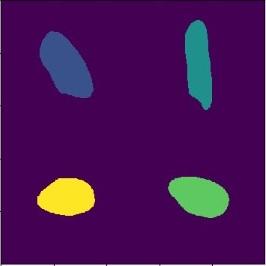
\includegraphics[height=2.9cm]{fg/spectral_clustering.jpg}
      \caption{}
      \label{fg:espectral_granos}
    \end{subfigure}
    \begin{subfigure}[c]{0.3\textwidth}
	   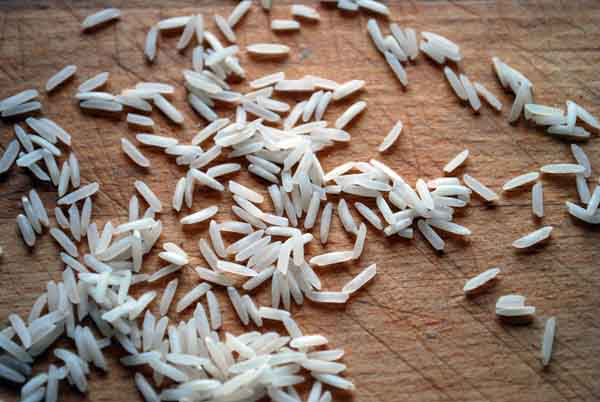
\includegraphics[width= 2.9 cm,height= 2.9 cm]{fg/muchos_basmati.jpg}
      \caption{}
      \label{fg:espectral_web}
	\end{subfigure}
	\begin{subfigure}[c]{0.3\textwidth}
	   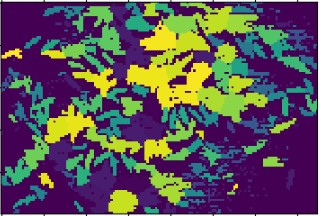
\includegraphics[width= 2.9 cm,height= 2.9 cm]{fg/muchos_basmati_spectral.jpg}
      \caption{}
      \label{fg:espectral_web_segmentada}
	\end{subfigure}
	\caption{Segmentaciones de imágenes mediante análisis espectral. a) Imagen sintética a partir del conjunto de datos de evaluación. b) Imagen obtenida de la web con muchos granos de arroz. c) Segmentación de la imagen de la web.}	
\label{fg:espectral}
\end{figure}


\section{Discusión y conclusiones}
En estudios anteriores sobre este mismo conjunto de datos se evaluaron algoritmos para la clasificación supervisada de imágenes de granos de arroz, ya sea directamente sobre las imágenes o previo procesamiento para extracción de atributos de tamaño, morfología y color. En contraste, en este trabajo se buscó evaluar el desempeño de algoritmos no supervisados de clustering en la tarea de separar las imágenes en grupos mapeables con las en variedades genéticas originales, partiendo de las imágenes. 
Para el caso de K-means y DBSCAN, las medidas de validación interna y externa no dieron un indicio claro de que el número de clusters óptimos correspondiera con el ńumero de variedades de arroz presentes en el conjunto de datos original. DBSCAN tuvo un desempeño muy pobre, posiblemente porque los puntos estaban distribuidos de forma homogénea en el espacio de atributos y DBSCAN se basa en contrastes de espacios de alta y baja densidad para realizar la agrupación y separación de los puntos. K-means y PAM tuvieron un mejor desempeño en términos de comparabilidad de la agrupación resultante con la clasificación original en variedades de arroz, siendo PAM ligeramente superior. No obstante, para los tres algoritmos la variedad Karacadag resultó ser la más distintiva, dada su forma redondeada. Tanto K-means como PAM agrupó casi la totalidad de estos granos en un cluster cuasi-exclusivo, separado de las otras variedades, mientras que ambos algoritmos tuvieron dificultad en separar entre sí las variedades alargadas, tanto las finas (Jazmín y Basmati) como las más robustas (Arborio e Ipsala).

En el caso de los algoritmos de segmentación, tanto CCL como clustering espectral presentaron resultados satisfactorios cuando los granos de arroz individuales se presentaban bien separados en la imagen. En cambio, para una imagen con gran cantidad de granos superpuestos, CCL no fue capaz de separar los granos ni siquiera en grupos más pequeños, mientras que el clustering espectral segmentó la imagen en conjuntos de granos más reconocibles. No se exploraron mayor cantidad de clusters objetivo para clustering espectral por limitaciones de tiempo, por lo que no se puede descartar que haya una versión del algoritmo que tenga un desempeño aún mejor que el evaluado aquí.

Por último, cabe destacar que este trabajo se realizó sobre una muestra pequeña de imágenes (5000) que resulta muy parecida al número de atributos alimentados a los algoritmos de clasificación, debido a que se trató de un trabajo preliminar. Esta línea de trabajo podría expandirse en el futuro a conjuntos de datos más nutridos que podrían resultar en agrupamientos no supervisados de mejor desempeño.


\printbibliography[title= Referencias, heading=bibintoc]

\end{document}
